% kuleuventheme2 by Janez Kren, September 2017, janez.kren@kuleuven.be, based on:
% kuleuventheme 1.3 by Roland Pastorino, 2013 roland.pastorino@kuleuven.be / www.rolandpastorino.com

\documentclass[11pt,t]{beamer}
\usetheme{kuleuven2}	%THEME OPTIONS for LOGO: kul (default), kulak, lrd,    ; OPTIONS for TITLE PAGE: normal (default), sedes


%%% OTHER SETTINGS
\usefonttheme[onlymath]{serif}			% math font with serifs, delete to make it sans-serif
\setbeamertemplate{footline}[body] 		% delete this line to remove footline bar on all frames
\usepackage[orientation=landscape,size=custom,width=16,height=9,scale=0.5,debug]{beamerposter} %enable for widescreen 16:9 ratio
%\titlegraphic{ \includegraphics[width=.2\paperwidth]{mytitlepagepic.png} } %optional title page image


%%% ADDED PACKAGES:
\usepackage[english]{babel}
\usepackage{amsfonts}
\usepackage{amssymb}


%%% TITLE PAGE INFO:
\title[Distributed Adversarial Attacks]{Distributed Adversarial Attacks} %[]] will appear in footline
\subtitle{Intermediate presentation}

\author{Sander Prenen}
\institute{KU Leuven}
\date{December 2021}




\begin{document}
\csname beamer@calculateheadfoot\endcsname %recalculate head and foot dimension

% Title page
\begin{frame}[plain,noframenumbering]
	\titlepage
\end{frame}

% Table of Contents
\begin{frame}{Outline}
	\hfill	{\large \parbox{.961\textwidth}{\tableofcontents[hideothersubsections]}}
\end{frame}

\section{Research topic}
\begin{frame}{Research topic}
\begin{itemize}
	\item Black-box adversarial attack
	\begin{itemize}
		\item Decision based
		\item No confidence scores
	\end{itemize}

	\item Distribution
	\begin{itemize}
		\item Particle swarm optimization (PSO)
	\end{itemize}
\end{itemize}
\end{frame}

\subsection{Related work}
%% Particle Swarm Optimization
\begin{frame}{Particle Swarm Optimization (PSO)}
\begin{itemize}
	\item Optimization framework
	\item Inspired by flocking of birds
	\begin{itemize}
		\item Each particle has a position and corresponding fitness
		\item Move based on personal best fitness, group best fitness and inertia 
	\end{itemize}
\end{itemize}
	\tikzset{every picture/.style={line width=0.75pt}} %set default line width to 0.75pt  
	      
\begin{figure}
\centering
\scalebox{0.5}{%
\begin{tikzpicture}[x=0.75pt,y=0.75pt,yscale=-1,xscale=1]

%uncomment if require: \path (0,300); %set diagram left start at 0, and has height of 300

%Shape: Circle [id:dp06935534605548432] 
\draw  [fill={rgb, 255:red, 0; green, 0; blue, 0 }  ,fill opacity=1 ] (100,161) .. controls (100,152.16) and (107.16,145) .. (116,145) .. controls (124.84,145) and (132,152.16) .. (132,161) .. controls (132,169.84) and (124.84,177) .. (116,177) .. controls (107.16,177) and (100,169.84) .. (100,161) -- cycle ;
%Straight Lines [id:da36297070749556615] 
\draw [color={rgb, 255:red, 255; green, 0; blue, 0 }  ,draw opacity=1 ][line width=3]    (116,161) -- (109.44,250.02) ;
\draw [shift={(109,256)}, rotate = 274.21] [fill={rgb, 255:red, 255; green, 0; blue, 0 }  ,fill opacity=1 ][line width=0.08]  [draw opacity=0] (16.97,-8.15) -- (0,0) -- (16.97,8.15) -- cycle    ;
%Shape: Circle [id:dp2975589876543052] 
\draw  [fill={rgb, 255:red, 0; green, 0; blue, 0 }  ,fill opacity=1 ] (258,156) .. controls (258,147.16) and (265.16,140) .. (274,140) .. controls (282.84,140) and (290,147.16) .. (290,156) .. controls (290,164.84) and (282.84,172) .. (274,172) .. controls (265.16,172) and (258,164.84) .. (258,156) -- cycle ;
%Straight Lines [id:da11974704599725938] 
\draw [color={rgb, 255:red, 255; green, 0; blue, 0 }  ,draw opacity=1 ][line width=3]    (274,156) -- (267.44,245.02) ;
\draw [shift={(267,251)}, rotate = 274.21] [fill={rgb, 255:red, 255; green, 0; blue, 0 }  ,fill opacity=1 ][line width=0.08]  [draw opacity=0] (16.97,-8.15) -- (0,0) -- (16.97,8.15) -- cycle    ;
%Straight Lines [id:da34669530870861953] 
\draw [color={rgb, 255:red, 0; green, 0; blue, 255 }  ,draw opacity=1 ][line width=3]    (267,251) -- (207.74,176.69) ;
\draw [shift={(204,172)}, rotate = 51.43] [fill={rgb, 255:red, 0; green, 0; blue, 255 }  ,fill opacity=1 ][line width=0.08]  [draw opacity=0] (16.97,-8.15) -- (0,0) -- (16.97,8.15) -- cycle    ;
%Straight Lines [id:da2944239439562262] 
\draw [color={rgb, 255:red, 55; green, 158; blue, 54 }  ,draw opacity=1 ][line width=3]    (204,172) -- (217.97,148.18) ;
\draw [shift={(221,143)}, rotate = 120.38] [fill={rgb, 255:red, 55; green, 158; blue, 54 }  ,fill opacity=1 ][line width=0.08]  [draw opacity=0] (16.97,-8.15) -- (0,0) -- (16.97,8.15) -- cycle    ;
%Straight Lines [id:da9472051718664152] 
\draw [color={rgb, 255:red, 243; green, 0; blue, 255 }  ,draw opacity=1 ][line width=2.25]  [dash pattern={on 2.53pt off 3.02pt}]  (274,156) -- (224.88,143.95) ;
\draw [shift={(221,143)}, rotate = 13.78] [color={rgb, 255:red, 243; green, 0; blue, 255 }  ,draw opacity=1 ][line width=2.25]    (15.74,-7.06) .. controls (10.01,-3.31) and (4.76,-0.96) .. (0,0) .. controls (4.76,0.96) and (10.01,3.31) .. (15.74,7.06)   ;
%Straight Lines [id:da8503925276289086] 
\draw [color={rgb, 255:red, 0; green, 0; blue, 255 }  ,draw opacity=1 ][line width=3]    (116,161) -- (56.74,86.69) ;
\draw [shift={(53,82)}, rotate = 51.43] [fill={rgb, 255:red, 0; green, 0; blue, 255 }  ,fill opacity=1 ][line width=0.08]  [draw opacity=0] (16.97,-8.15) -- (0,0) -- (16.97,8.15) -- cycle    ;
%Straight Lines [id:da10251717157021911] 
\draw [color={rgb, 255:red, 55; green, 158; blue, 54 }  ,draw opacity=1 ][line width=3]    (116,161) -- (129.97,137.18) ;
\draw [shift={(133,132)}, rotate = 120.38] [fill={rgb, 255:red, 55; green, 158; blue, 54 }  ,fill opacity=1 ][line width=0.08]  [draw opacity=0] (16.97,-8.15) -- (0,0) -- (16.97,8.15) -- cycle    ;

% Text Node
\draw (46,156) node [anchor=north west][inner sep=0.75pt]   [align=left] {Particle};
% Text Node
\draw (115,244) node [anchor=north west][inner sep=0.75pt]   [align=left] {\textcolor[rgb]{1,0,0}{Inertia}};
% Text Node
\draw (38,65) node [anchor=north west][inner sep=0.75pt]  [color={rgb, 255:red, 0; green, 0; blue, 255 }  ,opacity=1 ] [align=left] {Swarm best};
% Text Node
\draw (94,110) node [anchor=north west][inner sep=0.75pt]  [color={rgb, 255:red, 55; green, 158; blue, 54 }  ,opacity=1 ] [align=left] {Individual best};
% Text Node
\draw (212,117) node [anchor=north west][inner sep=0.75pt]   [align=left] {\textcolor[rgb]{0.95,0,1}{New position}};


\end{tikzpicture}
}
\caption{PSO logic, inspired by \cite{pso}}
\label{fig:pso}
\end{figure}


\end{frame}


%% Adversarial attack
\begin{frame}{Adversarial attack}
\vspace{-12pt}
	\begin{figure}
	\centering
	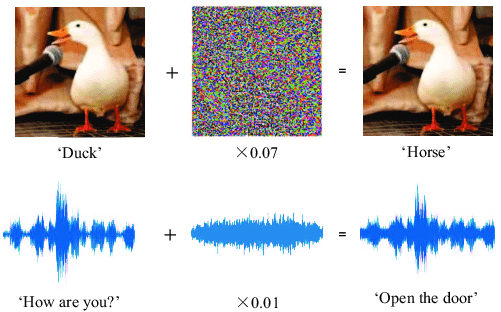
\includegraphics[width=0.6\textwidth]{graphics/adversarial_attack.png}
	\caption{Adversarial examples \label{fig:figure1} \cite{adversarial_attack}}
	\end{figure}
\end{frame}

\begin{frame}{Adversarial attack}
\begin{itemize}
	\item White box attack
	\begin{itemize}
		\item Access to output
		\item Access to model parameters
		\item Easier to attack
	\end{itemize}
	\item Black box attack
	\begin{itemize}
		\item Access to output
		\item \alert{No} access to model parameters
		\item More difficult to attack
		\item More relevant in real scenarios
	\end{itemize}
\end{itemize}
\end{frame}


%% Boundary Attack
\begin{frame}{Related work}
\begin{itemize}
	\item Boundary attack (BA)
	\vspace{6pt}
	\begin{figure}
	\centering
	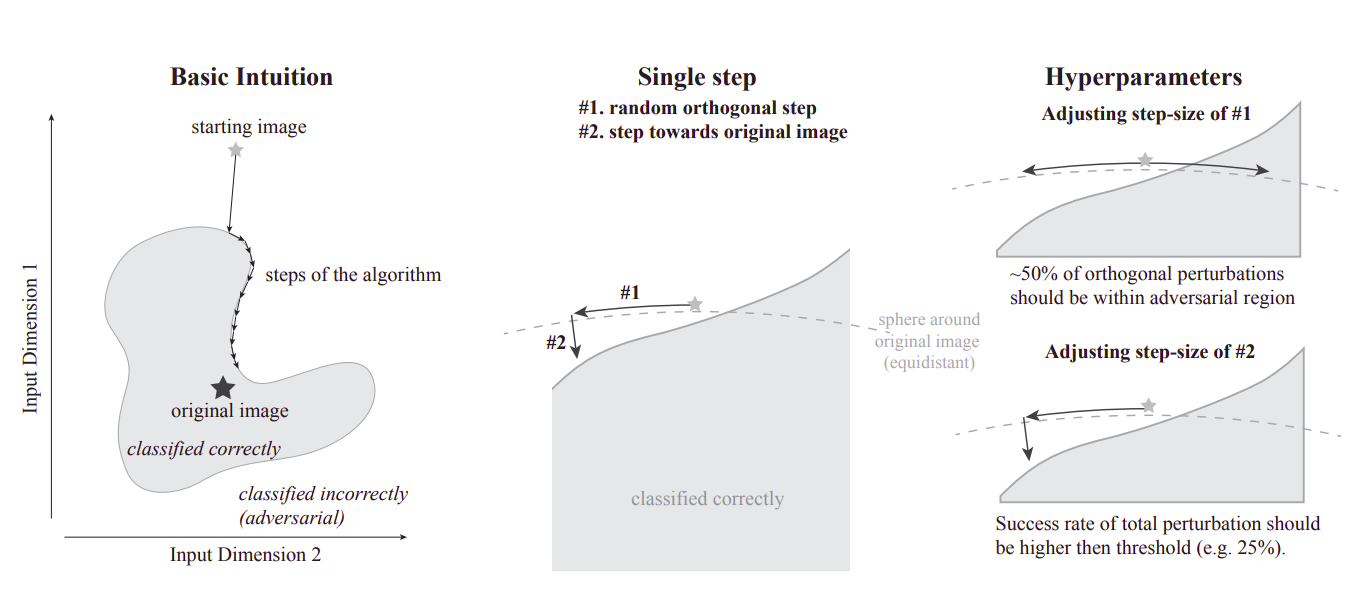
\includegraphics[width=0.8\textwidth]{graphics/boundary_attack.png}
	\caption{Boundary attack \cite{brendel2018decisionbased}\label{fig:boundary_attack}}
	\footnotesize
	\flushleft
	\end{figure}
\end{itemize}

\end{frame}

%%% Biased Boundary Attack
%\begin{frame}{Related work}
%\begin{itemize}
%	\item Boundary attack (BA)
%	\item Biased boundary Attack (BBA)
%	\begin{itemize}
%		\item Masking
%		\item Perlin noise
%	\end{itemize}
%\end{itemize}
%\end{frame}
%
%%% HopSkipJump Attack
%\begin{frame}{Related work}
%\begin{itemize}
%	\item HopSkipJump attack (HSJA)
%	\vspace{6pt}
%	\begin{figure}
%	\centering
%	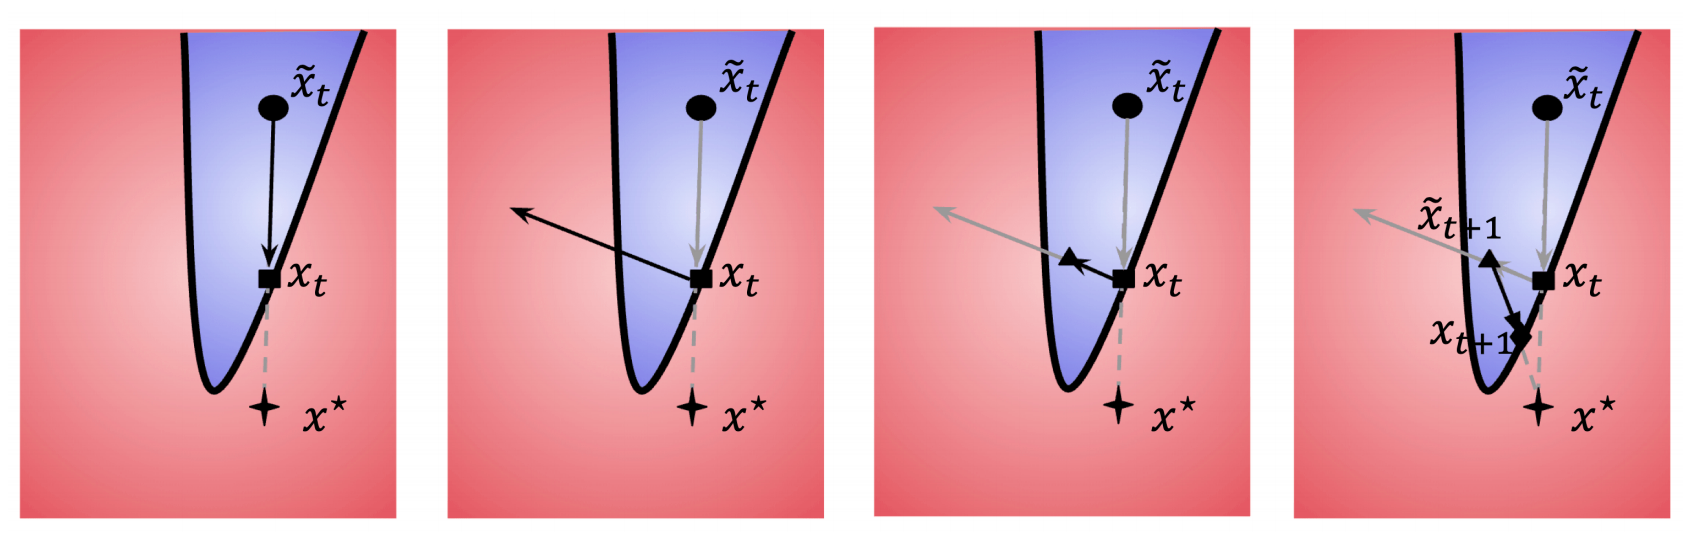
\includegraphics[width=0.8\textwidth]{graphics/hsj_attack.png}
%	\caption{HopSkipJump attack \cite{chen2020hopskipjumpattack}\label{fig:hsj_attack}}
%	\footnotesize
%	\flushleft
%	\end{figure}
%\end{itemize}
%\end{frame}

\subsection{Research gap}
\begin{frame}{Research gap}
\begin{itemize}
	\item Stateful detection
	\begin{figure}
	\centering
	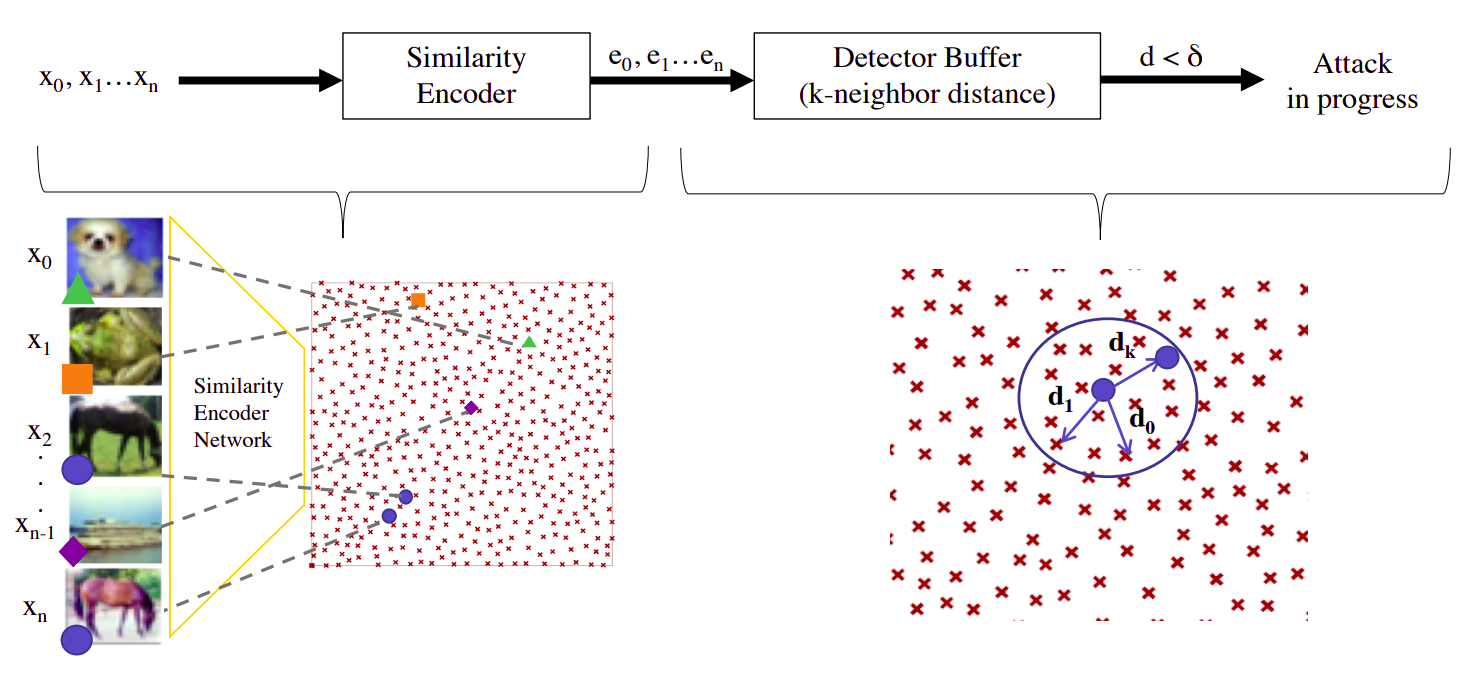
\includegraphics[width=0.8\textwidth]{graphics/stateful_detection.png}
	\caption{Stateful detection \cite{chen2019stateful}\label{fig:stateful_detection}}
	\footnotesize
	\flushleft
	\end{figure}
\end{itemize}
\end{frame}

\begin{frame}{Research gap}
\begin{itemize}
	\item Stateful detection
	\begin{itemize}
		\item Assumption: attack done by \alert{one} user/account/IP
		\item No cooperation between users
	\end{itemize}
	
	\item Distribution
	\begin{itemize}
		\item Evade the stateful detection algorithm
		\item Cooperate to craft better adversarial examples in fewer queries
	\end{itemize}
	
	\item Existing work
	\begin{itemize}
		\item Uses confidence scores \cite{10.1007/978-3-030-59013-0_22, s20247158}
	\end{itemize}
\end{itemize}
\end{frame}

\subsection{Research questions}
\begin{frame}{Possible research questions}
	\begin{exampleblock}
	{How can attackers cooperate in order to evade a stateful detection mechanism?}
	\end{exampleblock}
	\begin{exampleblock}
	{How can a single attacker distribute its queries in order to evade detection?}
	\end{exampleblock}
	\begin{exampleblock}
	{What are the advantages of distributing an adversarial attack?}
	\end{exampleblock}
	\begin{exampleblock}
	{What are to (dis)advantages of PSO in relation to adversarial attacks?}
	\end{exampleblock}
\end{frame}

\section{Progress}
\begin{frame}{Progress}
\begin{itemize}
	\item Working PSO algorithm based on boundary attack (PSO-BA)
	\begin{figure}
	\centering
	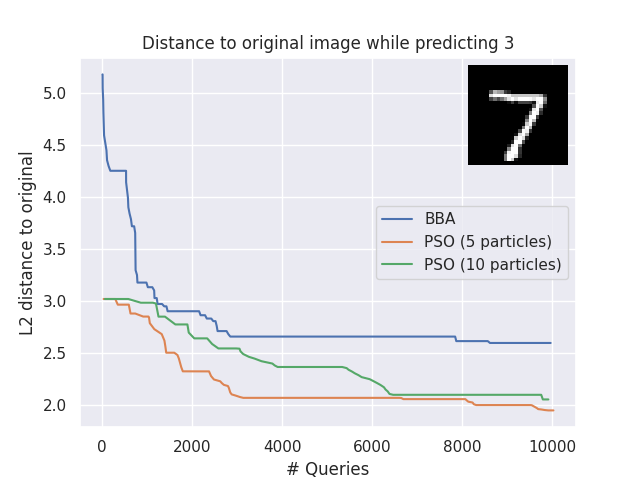
\includegraphics[width=0.30\textwidth]{graphics/comparison_1_3.png}
	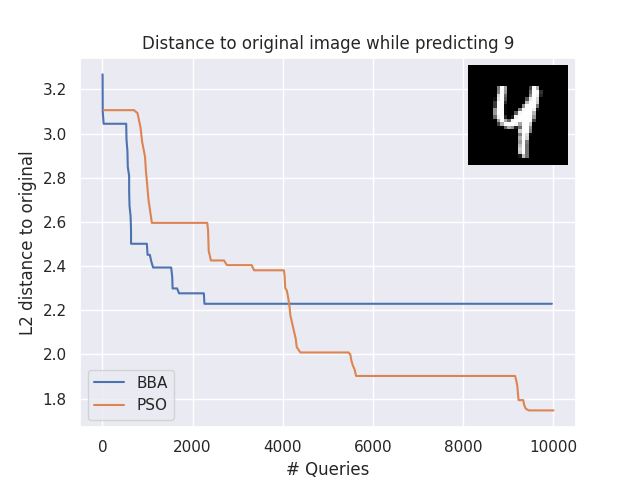
\includegraphics[width=0.30\textwidth]{graphics/comparison_42_9.png}
	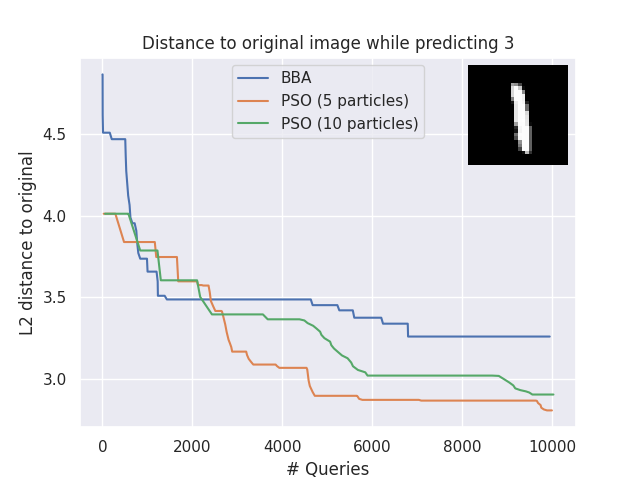
\includegraphics[width=0.30\textwidth]{graphics/comparison_1302_3.png}
	\caption{Comparison BA and PSO-BA\label{fig:comparisons}}
	\footnotesize
	\flushleft
	\end{figure}
\end{itemize}
\end{frame}

\begin{frame}[plain]{Progress}
\begin{itemize}
	\item Working PSO algorithm based on boundary attack (PSO-BA)
	\item Performed experiments to show that PSO is a viable candidate
	\begin{figure}
	\centering
	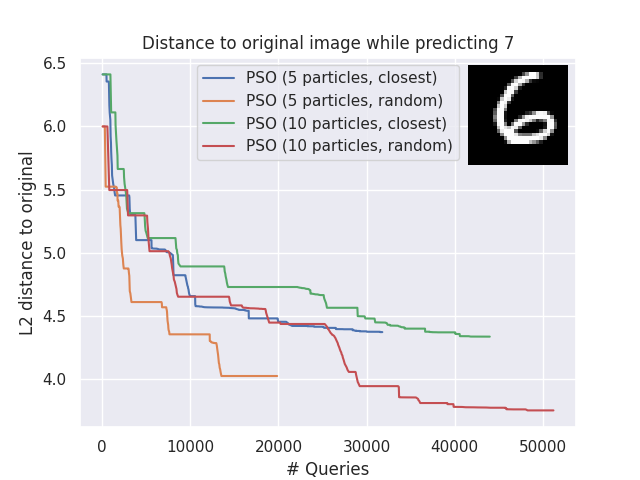
\includegraphics[width=0.45\textwidth]{graphics/random_vs_closest.png}
	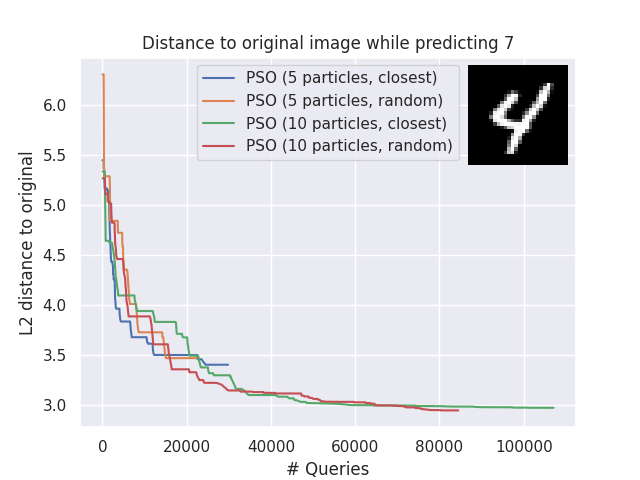
\includegraphics[width=0.45\textwidth]{graphics/random_vs_closest_1.png}
	\caption{Comparison random versus closest initialization\label{fig:rand_vs_close}}
	\footnotesize
	\flushleft
	\end{figure}
\end{itemize}
\end{frame}

\begin{frame}{Progress}
\begin{itemize}
	\item Working PSO algorithm based on boundary attack (PSO-BA)
	\item Performed experiments to show that PSO is a viable candidate
	\item Compare detections PSO-BA and BA (Not done yet but hopefully have done this before the presentation)
\end{itemize}
\end{frame}

\section{Future work}
\begin{frame}{Future work}
\begin{itemize}
	\item Improving the existing PSO-BA
	\begin{itemize}
		\item Implementing different distribution schemes and comparing the number of detections
		\item Tuning the hyperparameters to minimize detections
		\item Performing more experiments to confirm the results
		\item Applying the algorithm on different datasets
	\end{itemize}
	\item Implementing a new algorithm based on more efficient black box attacks (such as HopSkipJump attack)
	\begin{itemize}
		\item Comparing this algorithm with PSO-BA
	\end{itemize}
\end{itemize}
\end{frame}

\begin{frame}[c,plain,noframenumbering]
\begin{tikzpicture}[remember picture,overlay]
\fill[fill=kul-blue]
    (current page.south east)  rectangle  ([shift={(0,-0.1\paperheight)}]current page.north west)   ;
\end{tikzpicture}

\centering
\textcolor{white}{Questions?}
\end{frame}

\appendix
\section*{References}
\begin{frame}[allowframebreaks]{References}
\bibliographystyle{unsrt}
\bibliography{citations.bib}
\end{frame}
\end{document}
